\documentclass[aspectratio=169,10pt]{beamer}

\usetheme[
  color=red,
  font=lato,
  titlefont=avantgarde,
  footerlogo=hust,
  bar=thin,
  titlepage=cover,
  sectionpage=panel,
  numbering=fraction,
  progressbar=on,
  framebg=on
]{HUST}
\input{hust-setup}

\usepackage{amsmath,amssymb}
\usepackage{booktabs,graphicx,tabularx}
\usepackage[backend=biber,style=numeric,sorting=none,maxcitenames=2,mincitenames=1]{biblatex}
\addbibresource{references.bib}
\graphicspath{{figures/}{../../HUST-Beamer-Theme/assets/}}

\title[WEMoE for NLP]{Merging BERT Experts with Weight-Ensembling MoE}
\subtitle{Few-shot router training across five GLUE tasks}
\author[Group 1]{Group 1\texorpdfstring{\\[2pt]}{ }{\small Nguyễn Bá Anh -- 20261218M\\ Nguyễn Thị Nhã Linh -- 20261262M}\texorpdfstring{\\[2pt]}{ }{\small\textcolor{blue!55!black}{Instructor: Nguyễn Kiêm Hiếu}}}
\institute{}
\date{}
\hypersetup{pdfauthor={Nguyễn Bá Anh; Nguyễn Thị Nhã Linh; Instructor: Nguyễn Kiêm Hiếu}}

\begin{document}

\begin{frame}[plain]
  \titlepage
\end{frame}

\begin{frame}{Motivation: one model, many task experts}
  \begin{itemize}
    \item Fine-tuned experts retain task-specific performance, but five BERT-base checkpoints store \textbf{547.4M parameters}.
    \item Static merging is compact (Task Arithmetic: \textbf{57.4} average score) but loses much of the experts' performance.
    \item \textbf{Question:} can input-conditioned MLP weights recover task performance with one merged model, at lower storage than five experts?
  \end{itemize}
  \vfill
  \begin{block}{Scope}
    This is a BERT/GLUE adaptation of WEMoE, not a direct reproduction of the paper's CLIP/image experiments.\cite{tang2024wemoe}
  \end{block}
\end{frame}

\begin{frame}{Theory: route in task-vector space}
  For expert $e$, define its task vector relative to the pretrained weights:
  \[
    \tau_e = W_e - W_0.
  \]
  WEMoE constructs an input-conditioned MLP weight:
  \[
    W(x) = W_0 + \sum_{e=1}^{E} w_e(x)\,\tau_e.
  \]
  \begin{itemize}
    \item $W_0$ carries shared pretrained knowledge; $\tau_e$ captures an expert's task-specific change.
    \item The router weights $w_e(x)$ are \textbf{unnormalised}: they may amplify or subtract task vectors.
    \item This project adapts the weight-ensembling idea to BERT MLPs.\cite{tang2024wemoe}
  \end{itemize}
\end{frame}

\begin{frame}{Method: BERT MLPs become input-conditioned}
  \begin{itemize}
    \item Backbone: \texttt{bert-base-uncased}; experts fine-tuned separately for MRPC, RTE, CoLA, SST-2, and QNLI.
    \item For each BERT layer, a router uses the mean token representation over non-padding tokens to produce expert weights.
    \item Full scope ensembles both \texttt{intermediate.dense} and \texttt{output.dense}; intermediate-only ensembles the former.
    \item Other weights use Task Arithmetic ($\lambda=0.3$); task-specific classification heads are retained.
    \item FSFT trains only the routers (7.1M parameters); the backbone and the task experts stay frozen.
  \end{itemize}
  \vfill
  \centering
  \[
    \text{task experts}\longrightarrow\{\tau_e\}
    \longrightarrow\text{input router }w(x)
    \longrightarrow W(x)\text{ in each selected MLP}
  \]
\end{frame}

\begin{frame}{Data boundary: reserve router examples, select on dev}
  \centering
  \small
  \begin{tabularx}{\linewidth}{>{\bfseries}p{3.2cm} p{4cm} X}
    \toprule
    Portion of each official GLUE train split & Size & Used for\\
    \midrule
    \texttt{expert\_train} & Remaining examples & Fine-tune the task experts\\
    \texttt{fewshot\_pool} & 256 per task & FSFT router training only\\
    \texttt{dev} & 10\%, at most 1,000 & Choose expert epoch, $\lambda$, and router step\\
    Official validation & Task-specific & Final reported metrics only\\
    \bottomrule
  \end{tabularx}
  \vfill
  \begin{block}{Leakage control}
    Experts never train on the few-shot pool or dev split; official validation is not used for model selection.
  \end{block}
\end{frame}

\begin{frame}{Experiments: compare merging, routing, and expert limits}
  \begin{itemize}
    \item Five tasks: MRPC, RTE, CoLA, SST-2, QNLI; BERT-base with max sequence length 128.
    \item Baselines: majority prediction, simple averaging, Task Arithmetic ($\lambda$ chosen on dev), and separately fine-tuned experts.
    \item WEMoE uses $\lambda=0.3$ for its non-MLP merge and router initialization; FSFT trains the routers with labeled examples, selecting the best dev checkpoint every 50 steps (up to 500).
  \end{itemize}
  \vfill
  \begin{block}{Task score}
    MRPC: mean of accuracy and F1; CoLA: Matthews correlation (MCC); RTE, SST-2, QNLI: accuracy. Scores below are scaled by 100.
  \end{block}
\end{frame}

\begin{frame}{Main result: FSFT recovers much of the merging gap}
  \centering
  \begin{tabular}{l r}
    \toprule
    Model & Average task score\\
    \midrule
    Majority class & 45.8\\
    Simple Averaging ($\lambda=1/5$) & 53.3\\
    Task Arithmetic ($\lambda=0.3$) & 57.4\\
    WEMoE init (before FSFT) & 57.8 $\pm$ 0.6\\
    WEMoE + FSFT, full MLP ($k=256$) & \textbf{69.9 $\pm$ 0.1}\\
    Five single-task experts & 78.2\\
    \bottomrule
  \end{tabular}
  \vfill
  \begin{itemize}
    \item Gain over majority, (score $-$ majority)/(expert $-$ majority): Task Arithmetic \textbf{18\%}, WEMoE + FSFT \textbf{59\%}; Task Arithmetic predicts one class on MRPC and RTE.
    \item Router initialisation alone does not help (57.8): the gain comes from FSFT.
    \item Reported means and standard deviations are over router seeds 0, 1, and 2; they are not recomputed from the partial local raw runs.
  \end{itemize}
\end{frame}

\begin{frame}{Few-shot budget: $k=256$ is stable, small $k$ is not}
  \centering
  \begin{tabular}{r r r r}
    \toprule
    $k$ per task & Avg score & Gain over majority & CoLA MCC\\
    \midrule
    16 & 60.8 $\pm$ 2.7 & 25.5\% & 27.6 $\pm$ 14.1\\
    64 & 64.6 $\pm$ 3.7 & 46.7\% & 20.5 $\pm$ 17.8\\
    256 & \textbf{69.9 $\pm$ 0.1} & 59.1\% & 42.6 $\pm$ 0.9\\
    \bottomrule
  \end{tabular}
  \vfill
  \begin{itemize}
    \item Full-MLP WEMoE, reported means $\pm$ std over router seeds 0, 1, 2.
    \item Small budgets overfit early (best dev step 50--250 of 500) and vary strongly across seeds.
    \item The average moves 3.8 points from $k=16$ to $64$, but gain over majority almost doubles: part of the $k=16$ average is MRPC/RTE at their constant-guess level.
  \end{itemize}
\end{frame}

\begin{frame}{Per-task results: aggregate gains hide a task trade-off}
  \centering
  \scriptsize
  \begin{tabular}{l c c c c c}
    \toprule
    & MRPC acc/F1 & RTE acc & CoLA MCC & SST-2 acc & QNLI acc\\
    \midrule
    Majority & 68.4/81.2 & 52.7 & 0.0 & 50.9 & 50.5\\
    Full MLP, $k=256$ & 76.3 $\pm$ 4.5 / 83.9 $\pm$ 2.8 & 52.0 $\pm$ 4.4 & 42.6 $\pm$ 0.9 & 88.0 $\pm$ 0.5 & 86.7 $\pm$ 0.7\\
    Intermediate, $k=256$ & 66.5 $\pm$ 0.7 / 76.6 $\pm$ 1.0 & 59.0 $\pm$ 0.9 & 41.7 $\pm$ 0.9 & 86.7 $\pm$ 0.2 & 86.5 $\pm$ 0.2\\
    \bottomrule
  \end{tabular}
  \vfill
  \begin{alertblock}{Do not read the mean as universal dominance}
    Full-MLP WEMoE is below the RTE majority baseline (52.0 vs.\ 52.7). Intermediate-only improves RTE but is below the MRPC majority (66.5/76.6 vs.\ 68.4/81.2).
  \end{alertblock}
  \vspace{-2pt}
  {\scriptsize RTE (277) and MRPC (408) validation sets are small (standard error about 3 and 2 points), so part of the full vs.\ intermediate gap may be noise.}
\end{frame}

\begin{frame}{Storage trade-off: intermediate-only is smaller, not uniformly better}
  \centering
  \begin{tabular}{l r r r l}
    \toprule
    Deployment & Stored params & vs.\ five models & Avg score & Task contrast\\
    \midrule
    Five experts & 547.4M & 100\% & 78.2 & Strongest average\\
    WEMoE, full MLP & 400.0M & 73.1\% & 69.9 $\pm$ 0.1 & MRPC 76.3; RTE 52.0\\
    WEMoE, intermediate & 258.4M & 47.2\% & 69.1 $\pm$ 0.1 & MRPC 66.5; RTE 59.0\\
    \bottomrule
  \end{tabular}
  \vfill
  \begin{itemize}
    \item Intermediate-only stores about \textbf{35\% fewer parameters} than full-MLP WEMoE, at a similar reported average score.
    \item \textbf{Caveat:} each task keeps its own head, so the task is known at inference; five experts are then more accurate and only 37\% larger than full-MLP WEMoE. The storage case rests on the intermediate-only variant or on settings with unknown task.
    \item Intermediate-only reaches its best step late (400--500 of 500), so it may improve with more steps.
    \item Reported FSFT training estimates on one Tesla T4: about 14--16 minutes per full run vs.\ 8.5 minutes intermediate; hardware-specific, not inference latency.
  \end{itemize}
\end{frame}

\begin{frame}{Routing: shared structure, and why full-MLP fails on RTE}
  \centering
  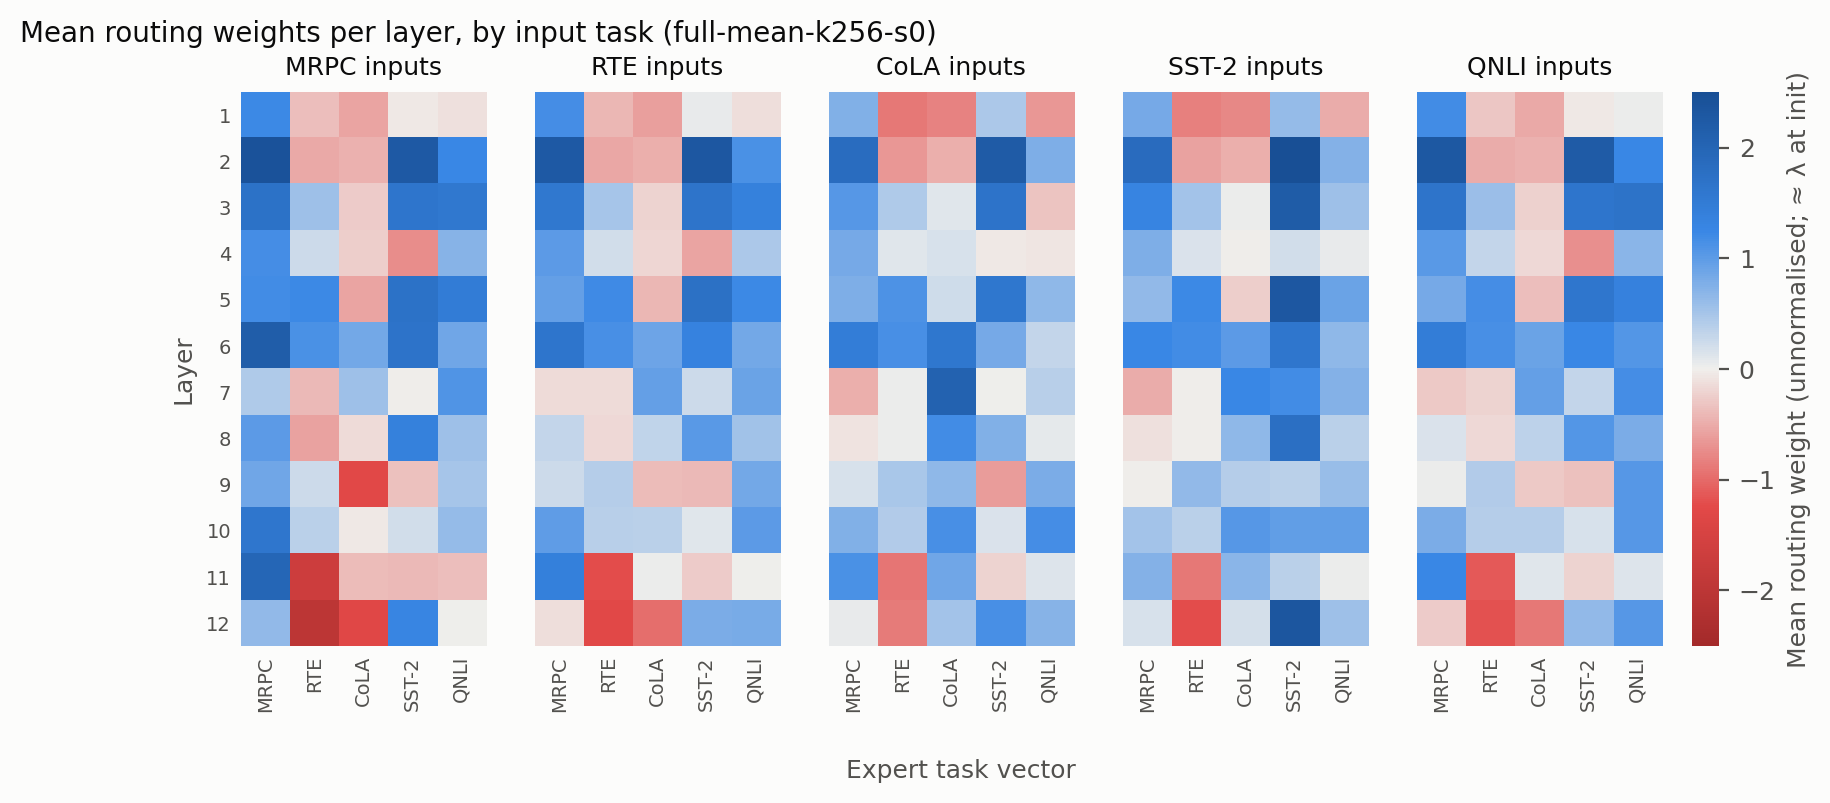
\includegraphics[width=0.96\linewidth,height=0.42\textheight,keepaspectratio]{routing.png}
  \vspace{-2pt}
  \begin{itemize}
    \item Similar patterns across input tasks: mean-matrix correlation 0.82; input task explains about 58\% of routing variance. Weights span $-3.0$ to $4.4$ (unnormalised).
    \item \textbf{RTE:} the full-MLP router gives the RTE task vector weight $\approx 0$ even on RTE inputs (own expert: 0.01, vs.\ 1.37 for MRPC) and subtracts it in layers 11--12 ($-1.2$). Intermediate-only gives it 0.96 on average and reaches 59.0.
  \end{itemize}
  {\scriptsize Report figure: full MLP, $k=256$, seed 0. The input-independent routing ablation is pending; this plot alone does not establish that input dependence causes the score gains.}
\end{frame}

\begin{frame}{Limitations: encouraging aggregate, unresolved failures}
  \begin{itemize}
    \item \textbf{RTE remains a failure case:} full MLP scores 52.0, below the 52.7 majority baseline; the underlying RTE expert is also relatively weak.
    \item \textbf{Small budgets are variable:} at $k=16$, CoLA MCC standard deviation is 14.1 across router seeds.
    \item \textbf{Selection sees more labels:} dev uses up to 1,000 examples per task, even when FSFT trains on only $k=256$.
    \item \textbf{Incomplete evidence:} experts/data split use one seed; local raw router results do not contain all seeds behind the report aggregates.
    \item \textbf{Efficiency gap:} inference latency and the input-independent ablation remain pending.
  \end{itemize}
  \vfill
  \centering
  \small The paper uses CLIP/image tasks and unlabeled test-time entropy minimisation for the router; here FSFT uses 256 labelled examples per task. Comparisons are qualitative.\cite{tang2024wemoe}
\end{frame}

\begin{frame}{Conclusion: WEMoE helps, but the task-level trade-offs matter}
  \begin{block}{Answer}
    In this first full BERT/GLUE run, few-shot router training raises the reported average to 69.9, recovering much of the gap left by static merging.
  \end{block}
  \begin{itemize}
    \item Full MLP and intermediate-only WEMoE reach similar averages with different storage and per-task outcomes.
    \item RTE remains below majority for full MLP; do not infer per-task dominance from an aggregate.
    \item More complete seeds, stricter few-shot model selection, the routing ablation, and measured inference latency are needed next.
  \end{itemize}
\end{frame}

\begin{frame}{Backup: task metrics and aggregation}
  \begin{itemize}
    \item \textbf{MRPC:} task score is the mean of accuracy and F1; the per-task table reports both values.
    \item \textbf{CoLA:} task score is Matthews correlation coefficient (MCC), not accuracy.
    \item \textbf{RTE, SST-2, QNLI:} task score is accuracy.
    \item \textbf{Average score:} unweighted mean of the five task scores; displayed on a $\times 100$ scale.
    \item \textbf{Uncertainty:} WEMoE results are reported as mean $\pm$ standard deviation over router seeds 0, 1, and 2; experts and data split are fixed.
  \end{itemize}
\end{frame}

\begin{frame}{Backup: router training details}
  \begin{itemize}
    \item The shared data split reserves 256 labeled examples per task for FSFT; experts never see those examples.
    \item Routers use two hidden layers, mean-pooled non-padding-token inputs, learning rate $10^{-4}$, and up to 500 update steps.
    \item The report counts 7.1M trainable router parameters; the pretrained backbone and task experts are not fine-tuned during FSFT.
    \item Best step is selected using dev evaluations every 50 steps; dev contains up to 1,000 examples per task.
    \item Reported figures are from the project's first full run, not a general performance guarantee or a complete reproduction of WEMoE.
  \end{itemize}
\end{frame}

\begin{hustreferencesframe}[title={References},subtitle={}]
\end{hustreferencesframe}

\end{document}
